\item Consider the matrix
$\vec{P} = \myvec{1 & 1 & 0 \\
                  0 & 1 & 1 \\
                  0 & 0 & 1} $.
The number of distinct eigenvalues of $ \vec{P} $ is
\begin{multicols}{4}
\begin{enumerate}
    \item 0
    \item 1
    \item 2
    \item 3
\end{enumerate}
\end{multicols}
\hfill (ME 2019)
\item The position vector $\overrightarrow{OP}$ of point $\vec{P}(20, 10)$ is rotated anti-clockwise in the $X-Y$ plane by an angle $\theta = 30\degree$ such that point $\vec{P}$ occupies position $\vec{Q}$, as shown in the figure. The coordinates $(x, y)$ of $\vec{Q}$ are
\begin{figure}[H]
\centering
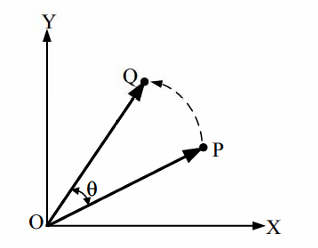
\includegraphics[width=0.5\textwidth]{GATE/2019/ME/figs/Fig 5.png}
\caption{}
\label{fig:question16}
\end{figure}
\begin{multicols}{4}
\begin{enumerate}
\item (13.40, 22.32) 
\item (22.32, 8.26)  
\item (12.32, 18.66)  
\item (18.66, 12.32)  
\end{enumerate}
\end{multicols}
\hfill (ME 2019)
\item The set of equations
\begin{align*}
x + y + z &= 1 \\
ax - ay + 3z &= 5 \\
5x - 3y + az &= 6
\end{align*}
has infinite solutions, if $ a =$\rule{1cm}{0.01pt}.
\begin{multicols}{4}
\begin{enumerate}
    \item -3
    \item 3
    \item 4
    \item -4
\end{enumerate}
\end{multicols}
\hfill (ME 2019)

